%# -*- coding: utf-8 -*-
%%% Local Variables:
%%% coding: utf-8
%%% mode:latex
%%% TeX-engine: xetex
%%% End:
%%采用 xelatex + ctex 文档类
\documentclass[fancyhdr,fntef,UTF8,oneside,12pt,a4paper, adobefonts]{ctexbook}
% \usepackage[adobefonts]{ctex} 
%%%%%!!!请将您的个人信息按照注释正确填写!!!%%%%%

%% Chinese
\newcommand{\department} {计算机科学与技术系}  	%院系
\newcommand{\major}      {计算机科学与技术} 	%专业方向
\newcommand{\thesistitle}{基于模拟退火算法的虚拟机部署技术} 	%论文题目
\newcommand{\grade}      {2008级}	    %年级
\newcommand{\NJUID}      {081221070}%学号
\newcommand{\myname}     {钱行}		%姓名
\newcommand{\advisor}    {钱柱中}		%指导老师姓名
\newcommand{\advisorjob} {副教授}		%指导老师职称
\newcommand{\enteryear}  {2008}		%入学年份

%% English
\newcommand{\edepartment} {Department of Computer Science}	%院系
\newcommand{\emajor}      {Computer Science}				%专业方向
\newcommand{\ethesistitle}{Solve Virtual Machine Placement Problem Using A Simulated Annealing Based Algorithm}			%论文题目
\newcommand{\emyname}     {Hang Qian}			%姓名
\newcommand{\eadvisor}    {Zhuzhong Qian}				%指导老师姓名
%% 字体设置

\setCJKfamilyfont{song}{Adobe Song Std}
\setCJKfamilyfont{zhongsong}{Adobe Song Std}
\setCJKfamilyfont{kai}{Adobe Kaiti Std}
\setCJKfamilyfont{hei}{Adobe Heiti Std}
\setCJKfamilyfont{fs}{Adobe Fangsong Std}
\setCJKfamilyfont{li}{Adobe Kaiti Std}
\setCJKfamilyfont{yy}{Adobe Fangsong Std}
\newcommand{\song}{\CJKfamily{song}}
\newcommand{\zs}{\CJKfamily{zhongsong}}
\newcommand{\kai}{\CJKfamily{kai}}
\newcommand{\hei}{\CJKfamily{hei}}
\newcommand{\fs}{\CJKfamily{fs}}
\newcommand{\li}{\CJKfamily{li}}
\newcommand{\yy}{\CJKfamily{yy}}
%\setmainfont{Arial}
% \renewcommand{\familydefault}{\sfdefault}
\setmainfont{Times New Roman} %英文字体使用Times New Roman
%\setmainfont[SmallCapsFont=LMRomanCaps10]{Times New Roman}
%Times New Roman 字体不包括 Small Caps 形状,如果要使用,需设定 Small Caps 字体,如 LMRomanCaps10

\renewcommand{\ULthickness}{0.7pt}
\newcommand{\myuline}[2]      {\uline{\makebox[#1]{#2}}}
\newcommand{\NJUTunderline}[1]{\uline{\hfill{#1}\hfill}}
\footnotesep=10pt


\usepackage{amsmath,amsfonts,amssymb}
\usepackage{array}
\usepackage{booktabs,multirow,colortbl,longtable,threeparttable}
\usepackage{verbatim}
\usepackage{lipsum}
\usepackage{comment}
\usepackage{footnpag}
\usepackage[ruled,vlined]{algorithm2e}


\usepackage{fontspec}


%% 加载图形宏包
\usepackage{graphicx}
%% 设置图片目录
\graphicspath{{figures/}}
\usepackage[config]{subfig}
\usepackage{indentfirst}
\usepackage[neverdecrease]{paralist}
\let\itemize\compactitem
\let\enditemize\endcompactitem
\let\enumerate\compactenum
\let\endenumerate\endcompactenum
\let\description\compactdesc
\let\enddescription\endcompactdesc

%%设置浮动体(表格、图片)标题格式
\DeclareCaptionLabelFormat{nju}{{\zihao{5}\song #1~#2}}
\DeclareCaptionLabelSeparator{nju}{\hspace{1em}}
\DeclareCaptionFont{nju}{\zihao{5}\song}
\captionsetup{labelformat=nju,labelsep=nju,font=nju}
\captionsetup[table]{position=top,belowskip={12bp-\intextsep},aboveskip=6bp}
\captionsetup[figure]{position=bottom,belowskip={12bp-\intextsep},aboveskip=6bp}

%% 超链接、目录
\usepackage{hyperref}
\usepackage{xcolor}
\definecolor{darkblue}{rgb}{0,0,0.55}
\hypersetup{CJKbookmarks,bookmarksnumbered,%
			colorlinks,unicode=true,%
			linkcolor=black,%
			citecolor=darkblue,%
			plainpages=false,%
			bookmarksopen=true,%
			bookmarksopenlevel=1,
			pdfstartview=FitH,
			pdftitle={\thesistitle},
    		pdfauthor={\myname},
    		pdfcreator={XeLaTeX with NJUThesis template designed by pkuphy},}
\usepackage{tabularx}%只要把tabularx包的引用放到hyperref包之后,正文脚注编号就能正常生成超链接。
%%版面控制
\usepackage{geometry}
\geometry{top=3.5cm,bottom=3.5cm,left=3.2cm,right=3.2cm}
%\geometry{headheight=2.6cm,headsep=5mm,footskip=13mm}
\parskip 0.5ex plus 0.25ex minus 0.25ex

\renewcommand{\textfraction}{0.15}
\renewcommand{\topfraction}{0.85}
\renewcommand{\bottomfraction}{0.65}
\renewcommand{\floatpagefraction}{0.60}


\fancypagestyle{myfancy}{%
\fancyhf{}
\fancyhead[C]{\small \song\leftmark}
\fancyfoot[C]{\small \thepage}
\renewcommand{\headrulewidth}{0.7pt}
}
\pagestyle{myfancy}


\setcounter{secnumdepth}{3}%%自动编号到 subsubsection

\CTEXsetup[nameformat={\hei\zihao{-2}}]{chapter}
\CTEXsetup[titleformat={\hei\zihao{-2}}]{chapter}
\CTEXsetup[beforeskip={-20pt}]{chapter}
\CTEXsetup[afterskip={20pt}]{chapter}
\CTEXsetup[format={\hei\zihao{-3}}]{section}
\CTEXsetup[nameformat={\bf\hei\zihao{-3}}]{section}
\CTEXsetup[beforeskip={-3ex plus -1ex minus -.2ex}]{section}
\CTEXsetup[afterskip={1.0ex plus .2ex}]{section}
\CTEXsetup[format={\hei\zihao{-4}}]{subsection}
\CTEXsetup[nameformat={\bf\hei\zihao{-4}}]{subsection}
\CTEXsetup[beforeskip={-2.5ex plus -1ex minus -.2ex}]{subsection}
\CTEXsetup[afterskip={1.0ex plus .2ex}]{subsection}
\CTEXoptions[contentsname={目\qquad 录}]
\CTEXoptions[listfigurename={插\qquad 图}]
\CTEXoptions[listtablename={表\qquad 格}]

%% 中文破折号,来自清华模板
\newcommand{\pozhehao}{\kern0.3ex\rule[0.8ex]{2em}{0.1ex}\kern0.3ex}
\newtheorem{defn}{\heiti 定义}[chapter]

\newenvironment{abstract}{
\thispagestyle{plain}
\pagenumbering{Roman}
\pdfbookmark[0]{中文摘要}{abstract}
\begin{center}
{\bf\kai\zihao{-2} \uuline{南~京~大~学~本~科~生~毕~业~论~文~中~文~摘~要}}
\end{center}
\bigskip

\noindent
\begin{minipage}{\textwidth}
\kai\zihao{4}%
\noindent{毕业论文题目:}\NJUTunderline{\thesistitle}\\
\NJUTunderline{\department}{院系}\NJUTunderline{\major}{专业}
\NJUTunderline{\enteryear}{级本科生}\hfill\\
{姓名:}\NJUTunderline{\myname}\\
{指导教师(姓名、职称):}\uline{\hfill\advisor 、\advisorjob\hfill}
\end{minipage}

\vskip 1cm
\begin{center}
{\heiti\zihao{-3} 摘\quad 要}
\end{center}\par
\kai\zihao{-4}
}{}
\newcommand\keywords[1]{\vspace{2ex}\noindent{\hei 关键词:} {\kai #1}}

\newenvironment{englishabstract}{
\clearpage
\thispagestyle{plain}
\pdfbookmark[0]{英文摘要}{englishabstract}
\begin{center}
{\bf\kai\zihao{-2} \uuline{南~京~大~学~本~科~生~毕~业~论~文~英~文~摘~要}}
\end{center}
\bigskip
\hyphenpenalty 10000
\noindent
{\zihao{4}%
\begin{description}
\item{THESIS:} {\bf\ethesistitle}
\item{DEPARTMENT:} {\bf\edepartment}
\item{SPECIALIZATION:} {\bf\emajor}
\item{UNDERGRADUATE:} {\bf\emyname}
\item{MENTOR:} {\bf\eadvisor}
\end{description}
}
\vskip 1cm
\begin{center}
{\bf\zihao{-3} Abstract}
\end{center}\par
}{}
\newcommand\englishkeywords[1]{\vspace{2ex}\noindent{\bf Keywords:} #1}

\renewcommand\maketitle{%
\clearpage
\thispagestyle{empty}
\pdfbookmark[0]{封面}{cover}

\begin{center}
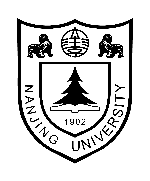
\includegraphics[width=1.96cm]{logo} \\
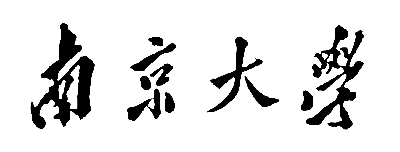
\includegraphics[height=2cm]{name} \\
\vskip 1cm
\zs
\zihao{0} 本~~科~~毕~~业~~论~~文\\
\vskip 2in\zihao{3}
\begin{minipage}{0.9\textwidth}
院\qquad 系\NJUTunderline{\department}\\[3mm]
专\qquad 业\NJUTunderline{\major}\\[3mm]
题\qquad 目\NJUTunderline{\thesistitle}\\[3mm]
年\qquad 级\myuline{4.5cm}{\grade}{\hfill}学\qquad 号\myuline{4cm}{\NJUID}\\[3mm]
学生姓名\NJUTunderline{\myname}\\[3mm]
指导老师\myuline{4.5cm}{\advisor}{\hfill}职\qquad 称\myuline{4cm}{\advisorjob}\\[3mm]
论文提交日期\NJUTunderline{2012年5月26日}
\end{minipage}
\end{center}
\clearpage
\thispagestyle{empty}
\vspace*{\stretch{1}}
{\kai\zihao{-3}
\noindent
\begin{tabular}{ccr}
\begin{CJKfilltwosides}{3.5cm}学号\end{CJKfilltwosides} & : & \makebox[6cm][r]{\NJUID}\\
\begin{CJKfilltwosides}{3.5cm}论文答辩日期\end{CJKfilltwosides} & : & \uline{2012}年\uline{5}月\uline{28}日\\
\begin{CJKfilltwosides}{3.5cm}指导教师\end{CJKfilltwosides} & : & \uline{\qquad\qquad\quad}(签字)\\
\end{tabular}
}
}

\newcommand\makeenglishtitle{%
\clearpage
\thispagestyle{empty}
\begin{center}
\vspace*{20pt}
\bf\zihao{2} \ethesistitle
\vskip \stretch{1}
\normalfont\zihao{4} by
\vskip 3pt
\bf\zihao{4} \emyname
\vskip \stretch{1}
\normalfont\zihao{4} Directed by
\vskip 3pt
\bf\zihao{4} \eadvisor
\vskip \stretch{2}
\normalfont\large \edepartment \\Nanjing University
\vskip 30pt
\CTEXoptions[today=old]
\normalfont\large May 26,2012
\vskip 20pt
\it\large Submitted in full fulfilment of the requirements\\for the degree of Bachelor of Science in Computer Science.
\end{center}
}


\usepackage{fontspec,xunicode,xltxtra}	% must be placed last

\begin{document} 
\maketitle
\makeenglishtitle

\frontmatter
\normalfont
\begin{abstract}
虚拟机部署问题是整个云计算的核心。能否高效率高性能的部署虚拟机请求和服务提供商的额成本和服务质量直接相关。虚拟机部署问题本质是一个多维装箱问题,该问题已经被证明属于NP-Hard问题。使用确定性算法解决虚拟机部署问题常常需要耗费大量的计算时间。本文描述了一种基于现实情境的部署需求,构造了一个基于模拟退火算法的启发式部署算法。从实验结果表明,本文方法在复杂需求下取得了比传统方法(FFD)更好的效果。
\end{abstract}

\keywords{云计算,虚拟机部署问题,模拟退火算法}

\begin{englishabstract}
The problem of virtual machine placement is at the core of cloud computing. The VM place problem is a reality extend of Bin Packing Problem, who had been proved to be NP-Hard problem. Using deterministic algorithms would cost vastly. In this paper, we proposed a modified Simulated Annealing alheuristic algorithm to solve a real-based VM placement problem. Experimental results shows that our methods achieves better performance than existing method on certain aspects.
\end{englishabstract}

\englishkeywords{Cloud Computing, Virtual Machine Placement,Simulated Annealing}
\clearpage

\pdfbookmark[0]{目录}{tableofcontents}
\tableofcontents
\listoffigures
%\listoftables  这条命令是表格目录,需要的话可以启用;上面那条是图片目录,不需要可以注释掉或者直接删除

\mainmatter
\zihao{-4}
\song


\chapter{引言}
\label{chap:1}

\section{云计算}
\label{sec:cloud-computing}

云计算(Cloud Computing)是这两年非``火热''一个概念。简单说,云计算是一种基于互联网的计算方式,通过这种方式,包括内存,计算能力(CPU资源),带宽等资源可以分配给有需求的用户。互联网上的云计算服务特征和自然界的云、水循环具有一定的相似性,因此,云是一个相当贴切的比喻。通常云计算服务应该具备以下几条特征:
\begin{itemize}
\item 基于虚拟化技术快速部署资源或获得服务
\item 实现动态的、可伸缩的扩展
\item 按需求提供资源、按使用量付费
\item 通过互联网提供、面向海量信息处理
\item 用户可以方便地参与
\item 形态灵活,聚散自如
\item 减少用户终端的处理负担
\item 降低了用户对于IT专业知识的依赖
\end{itemize}

云计算环境可以分为``软件即服务''(SaaS)、``平台即服务''(PaaS)、``架构即服务''(IaaS)。这些服务通过虚拟化技术提供给用户。目前比较有名的相关服务有Amazon EC2,GoGrid,Windows Azure和Rackspace Cloud。

\section{虚拟资源的部署}
\label{sec:virtual-machine-placement}

在云计算中,用户使用的是部署在一系列实体机之上的虚拟机,通常的实现形式是将虚拟机部署在大规模的计算集群中。在一台实体机(PM,下同)上可能存在多个虚拟机。因此,我们希望能够以最优的方式部署计算资源,从而尽可能的减少使用实体机的数量,达到节省成本(主要是能源成本)的目的。

在部署虚拟机湿,需要考虑的资源有实体机的内存、带宽、计算能力(CPU)等因素。这个问题可以被视为一个多维装箱问题(multi-dimensional vector bin packing problem)。VM所需要的资源被视为一个d维向量,其中每一维都是一个非负的值(即``小球'',一般取$0-1$的值);而每个PM所拥有资源也可以被看作一个d维向量,其中每一维,和VM的资源请求一样,代表一个独立的资源(即``箱子'',一般取值为$1$)。我们的目标是尽可能的减少``箱子''的数量并且能够满足将所有的VM请求部署在PM资源上且保证每个PM的上某一维上的请求都没有超过``箱子''的容量。因此,资源分配问题就可以视为一个d维装箱问题。




\section{问题定义}
\label{sec:prob-definition}

我们现在将所述问题进行数学定义:
\begin{defn}
\textbf{Vector Bin Packing problem}(VBP)


\label{VBP}

{\kai 给定一个有$n$个元素的$d$维向量的集合$S$,$S = \{\thinspace p_1,p_2,\cdots,p_n\ |\ p_i \in [0,1]^d \}$,寻找一个S上的划分$A_1,A_2,\cdots,A_m$使得$\sum_{p \in A_i}p^k\leq 1,\forall i,k$}
\end{defn}

VBP\ref{VBP}问题已经被证明是一个NP-Hard问题\cite{Garey76}。


\section{动机}
\label{sec:concern}


在很多企业提供的VPS(Virtual Private Server,虚拟专用服务器)服务中,提供给用户的选择很多都是不同的处理器性能和内存的大小。在实际的虚拟机部署中,除了资源分配的算法问题之外,还需要考虑如网络拓扑设计等许多方面的问题。但其中最关键也是最核心的问题还是如何根据用户的请求部署、移动虚拟机。在虚拟机部署考虑的资源中,计算资源和内部存储资源是最关键的,而外部存储资源(硬盘)等由于其成本相对较低,使用相对不频繁,因此通常并不做主要因素。

本文主要关注在理想环境下仅考虑计算资源(处理器核心)和内存的需求进行虚拟机部署的算法研究。



 








\chapter{相关工作}
\label{chap:2}

\section{虚拟机部署问题}

VM部署问题是整个云计算的一个基本问题,有很多研究都显示了合理部署VM的重要性\cite{Grit06}\cite{Bian04}。许多基于First Fit Decrease(FFD)的算法被应用在VM部署问题之中。Verma等\cite{Verm08}提出了一个能够通过尽量减少迁移\footnote{迁移是指对已经部署的虚拟机进行在其他实体机上再次部署的操作}达到最佳部署的方案。Hyser等\cite{Hyse07}提出了一个互动式的再部署方案,用以解决动态情境\footnote{动态情境指在算法开始前不能完全得知虚拟机请求的信息,需要根据实时信息进行部署的问题}下的问题。Bobroff等\cite{Bobr07}提出了一种预测请求并部署的动态规划算法。Shahabuddin等\cite{Shah01}提出了一种简单的启发式算法。

即使现阶段业界纷纷趋向虚拟化技术,VM部署问题仍研究尚浅。由于该问题的本质是一个NP-Complete问题,寻求最佳解效率比较低,为了克服这个问题,寻找一种效率较高并仍能获得比较好的结果的方法,我们提出了一个基于模拟退火算法,并能适应不同部署需求的算法。

\subsection*{模拟退火算法}
\label{sec:sa-inro}

模拟退火算法是一种基于概率的启发式算法,通常用来求解组合优化问题,寻找全局最优解。对于特定的问题,模拟退火的效率通常会优于全局搜索。Bohachevsky等证明,模拟退火算法依概率收敛到全局最优点。

模拟退火算法的名称来源冶金学专有的名词退火。退火是将材料加热后再以特定速率冷却,目的是增大结晶体的体积。我们将热力学的理论模拟至统计学上,将解空间内每一点想像成空气中的分子;分子的能量是它本身的动能,而解空间的每一点也像分子一样带有能量,以表示对命题的合适程度。算法先以搜寻空间内任意一点作起始,每一步先选择一个``邻居'',然后再计算从现有位置到达``邻居''的概率。

\subsection*{模拟退火算法在解决虚拟机部署问题时的优势}
\label{sec:advantage-of-sa}

对于VM部署问题,一个解可以被认为是单个VM状态的组合,算法的目标是对组合进行优化,寻找全局最优解。解的优劣可以用评价函数来体现。解的维度是虚拟机请求的规模,但是对于大规模的VM请求,解空间将变的巨大,经典的确定性算法将耗费巨大的计算时间和空间。使用启发式算法,特别是基于概率模型的模拟退火算法,可以有效的在巨大的解空间中快速逼近全局最优点。


\section{装箱问题}
VM部署问题的本质是装箱问题。一维装箱问题已经被深入研究。Fernandez de la Vega和Lueker\cite{Vega81}给出了首个线形时间逼近策略(APTAS)。他们的算法随后被Karmarker和Karp\cite{Karm82}改进,达到了$(1+log^2)$-\textsf{OPT}上界。

对于二维装箱问题,Woeginger\cite{Woeg97}证明了不存在APTAS。对于更高维的情况,Fernandez de la Vega和Lueker拓展了一维时的算法,提出了一种$(d+\epsilon)$-\textsf{OPT}的算法。Chekuri和Khanna\cite{Chan99}提出了一个$O(log~d)$近似算法,对于给定的$d$,算法运行在线形时间复杂度内。Bansal等\cite{Bans07}改进了这个结果,提出了一个对于任意$\epsilon \geq 0$的$(ln~d + 1 + \epsilon)$逼近算法。Karger等\cite{Karg07}提出了一种对于多维随机样例的VBP(Vector Bin Packing,向量装箱)问题使用技术的线形逼近方法。






\chapter{问题描述}
\label{chap:3}

\section{假设}
\label{sec:scenario}

在本文所关注的情境中,如上文\eqref{sec:concern}所说处理器资源(CPU,下同)和内存资源(RAM,下同)是我们考量的两个约束条件。

CPU资源和RAM资源在实际需求中具有不同的特点。

\subsection{CPU资源的特点}
\label{sec:cpu-character}

CPU资源具有原子性,即可以被分配的CPU资源一般是以计算核心(core)为单位的,而并非连续分配的。因此我们可以认为一台具有$N_{core}$个核心实体机的计算资源
\begin{equation}
  \label{eq:1}
C^{PM}=\{\ C^{PM}_1,C^{PM}_2,\cdots,C^{PM}_{N_{core}}\ \}  
\end{equation}

在通常情况下,集群中节点的每个计算核心的计算能力都是相同的,因此我们假设
\begin{equation}
  \label{eq:2}
C^{PM}=\{\ N_{core}\times C^{PM}_{core} \}  
\end{equation}

取$C^{PM}_{core} = 1$,则可以将一台实体机的计算资源$C^{PM}$由一个非负整数$N_{core}$来表示。同样,每个对计算资源的请求可以用一个非负实数$c_{req}$来表示。而由于CPU资源的原子性,每个CPU请求$c_{req}$应该分配$\lceil c_{req} \rceil $个核心。

\subsection{RAM资源的特点}
\label{sec:ram-character}

RAM资源具有可共享的特点,即多个虚拟机可以共享一段内存(严格的说,应当是分时的使用这一段内存,即在每一时刻如果某一段内存被一VM占用,则其他VM则不能访问这段内存)。在虚拟机资源的经典情境中,当一个PM尚未分配的RAM资源小于某一个VM的RAM请求时,该VM就不能被部署在这个PM上。而如果我考虑RAM资源可以被动态分配的特点,则可以满足PM上所有VM对RAM资源的请求总和大于该PM所拥有的RAM资源,即
\begin{equation}
\sum_{i}r^{req}_i \geq R^{PM}
\end{equation}
我们相信,这样的模型假设虽然简单,但是是合理的。比如在现代计算机系统中存在的虚拟内存就是内存可动态分配的一种体现。我们作出这样假设的前提是VM并不总是在使用它所请求的\textbf{所有}资源。所以,不可避免的,会出现一台PM上所有VM\textbf{实际使用的}RAM总和大于其所拥有的RAM总和,即$\sum_{i}r^{util}_i \geq R^{PM}$,我们称这样的情况为``冲突''。当冲突发生时,由于需要进行换页等操作来满足用户的需求,相当于牺牲了服务质量,可以认为付出了一定的代价。所有我们希望算法能够将此代价控制在一个阈值内。

所以,问题的输入为一个由资源请求组成的集合$V$,其每个元素由三个值组成$v_i = <c_i,r_i,\mu_i>$,分别表示对CPU资源和RAM资源的请求以及RAM资源的平均利用率。另有一个由PM资源组成的集合$P$,其每个元素为一个值对$p_j = <C,R>$,分别表示所拥有的CPU资源和RAM资源,且$C$,$R$均为常数;问题的输出是$V$上的一个划分,并且每一个划分都满足一定的条件。

\subsection{评价函数}
\label{sec:value-function}

在使用启发式算法求解问题时,需要对解空间内的每个解进行评价(Value),并根据评价来确定解的优劣。在经典的装箱问题中,求解的目标是尽可能的减少使用实体机的数量,因此计算一个解中使用PM的数量(即产生划分的个数)可以作为评价函数。

经典的装箱问题中,希望尽可能减少``箱子''数量的原因是为了降低成本。但是我们注意到,减少使用的PM数量所减少的成本通常是能源成本。而一个计算集群的成本还与服务质量有关,比如通信的质量,故障率等因素。在本文所描述的情境中,我们希望能同时关注成本与性能的问题。

我们定义了以下三方面的问题:

\begin{itemize}
\item \textbf{降低成本}。与经典的装箱问题相同,我们希望部署的结果在保证质量的前提下能尽可能的降低成本,即减少PM的使用。一台PM产生的成本,取决于是否有虚拟机被部署于其上,而可以认为与其上的负载没有关系(即一旦启动则认为成本一定),所以我们仍旧采用计算PM的数量来作为衡量解优劣的指标。
\item \textbf{负载均衡}。对于需要相互通信的计算集群(比如Hadoop集群),如果单个节点上的负载过高,则有可能会成为整个系统的性能瓶颈。我们希望部属的结果能尽可能的保证每个节点上的负载相对均衡。
\item \textbf{减少冲突}。由于我们采用了可以共享内存的模型,所以会出现一台PM上部署的VM的RAM请求之和大于PM自身拥有的RAM总和,因此有一定概率出现``冲突''的情况。我们希望部属的结果能尽可能的保证整个系统的冲突概率尽可能的减少。
\end{itemize}

由于这三方面的问题都和具体的应用情境相关,因为我们无法给出之间的具体权重。我们将会单独对三方面问题进行讨论,然后再对综合情况的结果加以探讨,以期给出一个相对开放的结论。

\section{虚拟机部署问题}
\label{sec:formulation}

下面对虚拟机部署问题基于上述假设描述的情境进行形式化。

\subsection*{变量表}
\label{sec:notation-table}

\begin{table}[htbp]

  \centering
  \begin{threeparttable}
    \caption{\label{tab:notation}变量表}
    \begin{tabular}{cl}
      \toprule
        变量名  &  说~明  \\
      \midrule
        $x_{ij}$    &  $VM_i$是否装入$PM_j$    \\
        $N_v$      &  虚拟机的数量    \\
        $N_p$      &  实体机的数量    \\
        $VM_i$     &  虚拟机请求$i$  \\
        $PM_j$     &  实体机$j$     \\
        $C^{req}_i$  &  $VM_i$的CPU请求 \\
        $R^{req}_i$  & $VM_i$的RAM请求 \\
        $ER_i$  & $VM_i$的RAM平均使用率 \\
        $C^{used}_j$  & $PM_j$已被分配的CPU \\
        $R^{used}_j$  & $PM_j$已被分配的RAM \\
        $C^T$       & $PM_j$所拥有的CPU \\
        $R^T$       & $PM_j$所拥有的RAM \\
      \bottomrule
    \end{tabular}
    \tiny
    \begin{tablenotes}
    \item [*] $x_{ij}$为一位二进制变量
    \item [**]$N_p$理想情况下应为无穷大
    \end{tablenotes}

  \end{threeparttable}
\end{table}

\subsection*{约束条件}
\label{sec:constraints}
上述变量\eqref{tab:notation}应当满足如下的约束条件:

\begin{eqnarray}
  \label{eq:constraints}
  N_v &\leq& N_p \label{eq:con:1}\\
  x_{ij} &=& \{\ 1,0\ \} \label{eq:con:2}\\
  \sum_j x_{ij} &=& 1 \label{eq:con:3} \\
  \sum_i C^{req}_i x_{ij} &\leq& C^T , \forall j \label{eq:con:4}\\
  \sum_i R^{req}_i\ ER_i\  x_{ij} &\leq& R^T , \forall j \label{eq:con:5}
\end{eqnarray}

这些约束条件的涵义如下:

\begin{itemize}
\item 公式~\eqref{eq:con:1}说明系统可以提供的PM的数量总多于VM的请求数\footnote{在实际情境中,虚拟机数量一般大于最终使用的实体机数量。实际上,我们应当定义实体机数量趋近无穷($0 \leq N_p \rightarrow +\infty$),即不对实体机数量作约束。而在算法实现中,我们需要保证算法能够产生至少一个有效解,因此约定$N_v \leq N_p$,并且在后文的实现中取不同的数据规模进行分析。}  
\item 公式~\eqref{eq:con:2}表示一个VM请求的两种状态:1表示被部署在$PM_j$中,0表示没有被部署在$PM_j$中

\item 公式~\eqref{eq:con:3}说明一个VM能且只能被部署在一个PM上。

\item 公式~\eqref{eq:con:4}和公式~\eqref{eq:con:5}说明每一个PM上所有VM的资源请求不能超过自身所拥有资源\footnote{注意到公式~\eqref{eq:con:5}限制每个PM上的所有VM的\textbf{平均}RAM资源请求,是因为RAM的可以共享性质。所以实际解中是会出现$\sum_i R^{req}_i x_{ij} \geq R^T$的情况的。}
\end{itemize}


\subsection*{目标}
\label{sec:objective}
算法的目标是找到这样的一个解:在满足上述约束条件的限制下,评价尽可能``低''\footnote{这里使用``低''是指采用的评价函数的值尽可能的小。由于本文采用的是模拟退火算法求解,评价函数的值越低表明系统的能量越小,即更靠近最优解。}。由于我们将会讨论多个评价函数下算法的表现,因此用$value(s)$表示对解$s$的评价。





\chapter{算法的设计与实现}
\label{chap:algo}

\section{设计}
\label{sec:design}
模拟退火算法是一个可以被高度抽象的算法。它的设计并不受制于所需要求解的问题(但是参数的设置需要根据问题的性质来设定)。我们设计的算法主要框架如下:

\begin{algorithm}[H]
  \DontPrintSemicolon
  \SetKwInOut{Input}{INPUT}
  \SetKwInOut{Output}{OUTPUT}
  \SetKwData{Temp}{temperature}
  \SetKwData{CurS}{cur\_state}
  \SetKwData{CurV}{cur\_value}
  \SetKwData{Neigh}{neighbor}
  \SetKwData{NewV}{new\_value}
  \SetKwData{Term}{term}
  \SetKwFunction{GetV}{value}
  \SetKwFunction{GetNeigh}{get\_neighbor}
  \SetKwFunction{Acc}{accept}
  \SetKwFunction{Cool}{cooldown}
  
  \Input{List $si$ which is a permutation of ids of PMs}
  \Output{List $so$ which is another permutation of ids of PMs}
  \Begin{
    \CurS$\leftarrow si$\;
    \CurV$\leftarrow$ \GetV{$si$}\;
    \Temp$\leftarrow$ $InitTemperature$\;
    \Term$\leftarrow$ $0$\;
    \While{$\Term < maxTerm \And \Temp > minTemperature $}
    {
      \Neigh $\leftarrow$ \GetNeigh{\CurS}\;
      \NewV $\leftarrow$ \GetV{\Neigh}\;
      \If{\Acc{\CurV,\NewV,\Temp}}
      {
        \CurS $\leftarrow$ \Neigh\;
        \CurV $\leftarrow$ \NewV\;
      }
      $\Term \leftarrow \Term + 1$\;
      \Temp $\leftarrow$ \Cool{\Temp,\Term}\;
    }
    \Return \CurS
  }
  \caption{Simulated Annealing\label{algo:SA}}
\end{algorithm}

算法的输入是一个``状态''$S$,表示形式为一个列表,表中的元素$S_i$表示$VM_i$被部署到$PM_{S_i}$。一个状态即代表问题的一个解。

算法的输出同样是一个状态,这是经过模拟退火算法迭代过后的新状态,它收敛到一个局部最优解。

\subsection{初始化}
\label{sec:init}

由于算法对初始状态并不敏感,因此我们采用了\texttt{random\_fit}的方法生成初始状态,其算法描述如下:

\begin{algorithm}[H]
  \DontPrintSemicolon
  \SetKwInOut{Input}{INPUT}
  \SetKwInOut{Output}{OUTPUT}
  \SetKwData{St}{state}
  \SetKwData{Pl}{plist}
  \SetKwData{PIndex}{pi}
  \SetKwData{PData}{p}
  \SetKwFunction{Random}{randomInt}
  \SetKwFunction{Avail}{available}
  \SetKwFunction{Assign}{assign}
  \SetKwFunction{Len}{length}
  
  \Input{List $V$ which is the VMs\' requests infomation}
  \Output{List $s$ which is a state(solution)}
  \Begin{
    \St $\leftarrow$ [~]\;
    \Pl $\leftarrow EmptyPmInfoList$ \;
    \For{$every vm_i \in V$}
    {
      \PIndex $\leftarrow$ \Random{0,\Len{\Pl}}\;
      \PData $\leftarrow$ \Pl[\PIndex]\;
      \Repeat{$available(vm_i,\PData)$}{
        \PIndex $\leftarrow$ \Random{0,\Len{\Pl}}\;
        \PData $\leftarrow$ \Pl[\PIndex]\;
      }
      \Assign{$vm_i$,\PData}\;
      \St[$i$] $\leftarrow$ \PIndex\;
    }
    \Return \St\;
  }
  \caption{Random Fit\label{algo:rf}}
\end{algorithm}

算法\ref{algo:rf}随机的在提供的PM序列里寻找可以(满足约束条件)部署的节点。直到所有VM均被成功部署后返回解状态。

\subsection{找寻邻解}
\label{sec:neighbor-algo}
算法\ref{algo:SA}中使用的\texttt{get\_neighbor(state)}过程用来从当前状态生成一个相邻的状态,找寻邻解的算法描述如下:

\begin{algorithm}[H]
  \DontPrintSemicolon
  \SetKwInOut{Input}{INPUT}
  \SetKwInOut{Output}{OUTPUT}
  \SetKwData{St}{state}
  \SetKwData{NewSt}{neighbor}
  \SetKwData{Src}{src}
  \SetKwData{Des}{des}
  \SetKwData{Pl}{plist}
  \SetKwData{PIndex}{pi}
  \SetKwData{PData}{p}
  \SetKwData{VData}{v}
  \SetKwData{Max}{max}
  \SetKwFunction{Random}{randomInt}
  \SetKwFunction{Avail}{available}
  \SetKwFunction{Assign}{assign}
  \SetKwFunction{Len}{length}
  
  \Input{Current state $s$}
  \Output{Neighbor state $neighbor$}
  \Begin{
    \NewSt $\leftarrow$ \St\;
    \For{$0$ \KwTo \Max }
    {
      \Src $\leftarrow$ \Random{0,$N_v$} \;
      \Des $\leftarrow$ \Random{0,$N_p$} \;
      \VData $\leftarrow VM_{\Src}$\;
      \PData $\leftarrow PM_{\Des}$\;
      \Repeat{\Avail{\VData,\PData}}
      {
        \Des $\leftarrow$ \Random{0,$N_p$} \;
        \PData $\leftarrow PM_{\Des}$\;
      }
      \NewSt[~\Src] $\leftarrow$ \Des\;
    }
    \Return \NewSt\;
  }
  \caption{Get Neighbor\label{algo:neighbor}}
\end{algorithm}

在算法\ref{algo:neighbor}中,我们对当前状态中的$max$个值进行了重新随机部署,$max$的取值决定了生成的邻解和当前解的距离。在模拟退火算法中,我们希望邻解有较高的随机性但是与当前解的距离不能太远,因此在实现中通常选$\frac{1}{10}$比例的值。

\subsection{接受条件}
\label{sec:accept}
算法\ref{algo:SA}中使用的\texttt{accept(cur,new,t)}用来判断是否接受当前邻点。根据Metropolis准则,金属粒子在温度T时趋于平衡的概率为$e^{-\frac{\Delta E}{KT}}$,其中K是Boltzmann常数。本文所使用的策略即来自这一准则,算法的描述如下:
\begin{algorithm}[H]
  \DontPrintSemicolon
  \SetKwInOut{Input}{INPUT}
  \SetKwInOut{Output}{OUTPUT}
  \SetKwData{CV}{cur}
  \SetKwData{NV}{new}
  \SetKwData{Del}{delta}
  \SetKwData{Tem}{t}
  \SetKwData{True}{true}
  \SetKwData{False}{false}
  \SetKwFunction{Random}{random}
  
  \Input{Current value \CV, neighbor value \NV, current temperature \Tem }
  \Output{Boolean value indicates accept neighbor or not}
  \Begin{
    \Del $\leftarrow \NV - \CV$\;
    \If{$\Del < 0$}{
      \Return \True\;
    }
    \Else
    {
      \If{$e^{-\frac{\Del}{t}} > \Random{0,1}$}
      {
        \Return \True\;
      }
    }
    \Return \False
  }
  \caption{Accept\label{algo:accept}}
\end{algorithm}
在上述算法\ref{algo:accept}中,\texttt{random(a,b)}函数随机返回一$a$到$b$之间的实数。

\section{实现}
\label{sec:implementation}

我们使用了Python编程语言对算法进行了实现。下面介绍一些值得注意的部分。

\subsection{参数的设置}
\label{sec:config}

模拟退火算法对参数设置是非常敏感的,包括初始温度的设置,降温的速度,评价函数的设计都会对最后收敛的速度和结果有比较大的影响。经过反复试验,我们确定了以下的参数设置:

\begin{itemize}
\item \textbf{初始温度}。由于在判断是否接受时计算了$\Delta value/t$的值,因此我们希望能将温度和评价归一化。初始温度被设置为初始评价的$K$倍,$K = N_v N_p$。
\item \textbf{降温速度}。降温速度太快会导致算法很快收敛,得不到比较理想的结果,而降温速度太慢则会导致收敛过程很长,并且在计算初期接受过于不理想的结果,影响效率。经过试验,使用了$t_{n+1} = 0.89t_n$这样的线形降温速度,收到了良好的效果。
\item \textbf{评价函数}。在实现中采用了四种因素综合评价的方式。我们考虑了PM的数量,RAM的负载均衡,CPU的负载均衡和平均冲突率,并以这四个值的乘积作为评价函数的返回值。\label{evalutation}
\end{itemize}

\subsection{评价函数}
\label{sec:evaluation-function}

在所有参数中,评价函数的确定是对算法影响最大的,因为它直接决定了算法的走向。比如我们选取使用PM的数量作为评价的标准,那么在迭代的过程中接受那些使用更少PM的解。如前文\ref{evaluation}所说,我们希望综合考虑更重因素,所以我们采用了如下的评价函数:

\begin{itemize}
\item \textbf{PM的数量}。我们用\texttt{count\_active(plist)}函数来评价。函数接受一个根据状态生成的PM信息列表,计算其中被``激活''(有VM部属在其上)的PM的个数(为了不同规模数据间的比较,实际返回的是PM的个数与$N_v$的比例。
\item \textbf{RAM的均衡负载}。我们用\texttt{ram\_stdev(plist)}函数来评价。函数接受一个根据状态生成的PM信息列表,计算RAM利用率的均方差(Standard Deviation)。如果RAM利用率的均方差的足够小则说明每台PM上的RAM负载比较均衡。
\item \textbf{CPU的均衡负载}。和RAM的均衡负载类似,我们用\texttt{cpu\_stdev(plist)}函数来评价。函数接受一个根据状态生成的PM信息列表,计算CPU利用率的均方差。如果RAM利用率的均方差的足够小则说明每台PM上的CPU负载比较均衡。
\item \textbf{平均冲突率}。我们定义平均冲突率$\mu \geq 1$,使用\texttt{count\_conficts(plist)}函数来计算。函数接受一个根据状态生成的PM信息列表,结算其中RAM利用率超过$1$的PM的平均RAM利用率。如果不存在利用率超过$1$的PM,则取值$1$.
\end{itemize}

\subsection{测试数据的选取}
\label{sec:data}
通常,云计算服务提供商提供的用户的选择都是有限的,比如提供给用户选择``双核500MB内存'',通过限制虚拟机请求的数据可以针对性的优化部属算法。在这种情境下,\texttt{First-Fit}算法通常能收到良好的效果。

在本文所描述的情境中,为了更好的模拟不同情境下算法的效果,我们没有对请求的数据进行限制(但是为了避免无解的情况,对数据的上下限进行了规定)。我们尝试了多种测试数据生成的方法,最终确定以下的测试数据:
\begin{itemize}
\item 每组测试设计都是\textbf{随机}生成的。
\item 将$C^T$设置为$8$,即认为每个实体机都具有$8$个计算核心;将$R_T$设为$1$。
\item $C^{req}_i$将取$0.1-8.0$之间的随机数;$R^{req}_i$取$0.2-0.8$之间的随机数;$ER_i$取$0.2-0.8$之间的随机数。生成的数据可以认为即包含运算需求高的请求也包含存储需求高的请求。
\item 测试数据的数量取$100-1000$间隔$100$的整数,用以模拟不同规模下的请求。
\end{itemize}

在随机的数据和不同的数据规模上的得到相似测试结果可以从某种程度上证明算法的稳定性和可行性。


\chapter{实验结果与结论}
\label{chap:result}
通过不同数据规模和多次试验,我们得出了相应的结论,并且与\texttt{First-Fit}算法在同样的数据上的结果进行了比对。

\section{有效性}
下图\ref{fig:feas}是算法在$N_v = 200,N_p = 200$时的迭代情况,我们看到在算法最终收敛在一个比较好的解上。在所有测试中算法均能成功收敛在一个解上。
\begin{figure}[htbp]
\centering %图形居中
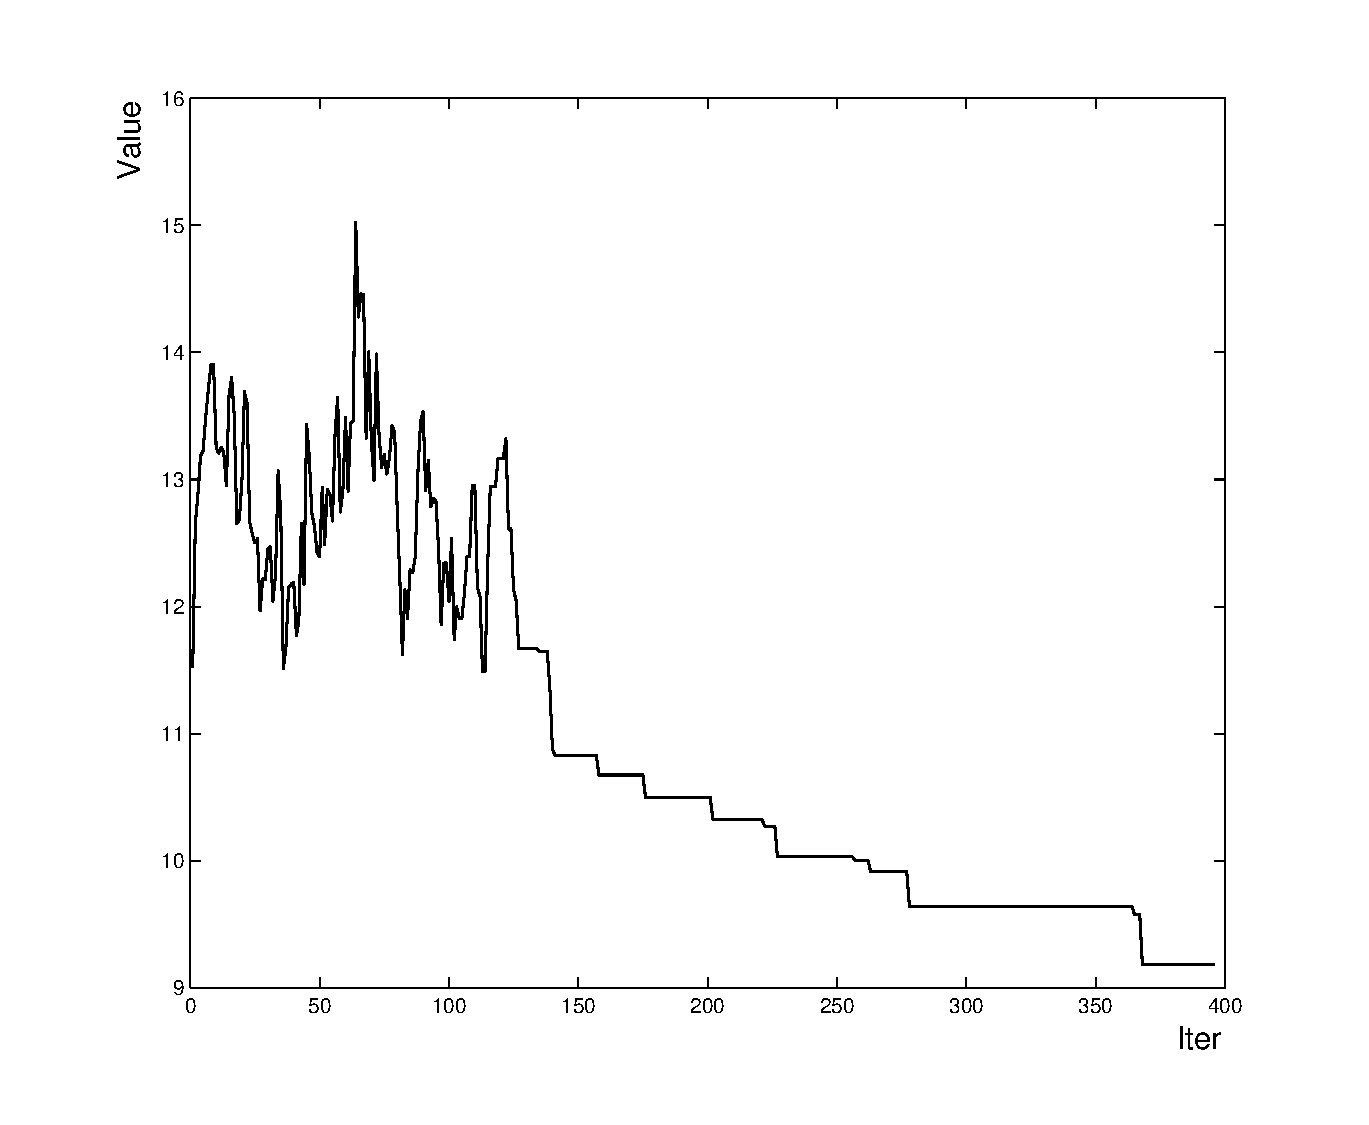
\includegraphics[width=0.8\textwidth]{figures/feasibility.eps}
\caption{算法收敛} \label{fig:feas}
\end{figure}
\section{稳定性}
我们已经看到算法可以成功收敛,但是如果每次收敛的结果差距过大则说明算法并不稳定,即不能保证每次都能得到一个较好的解。从下表\ref{tab:stability}我们可以看到,当取$N_v = 100, N_p = 100$时,十组不同数据的测试最终收敛的结果非常相近,并且都是较好的解。说明算法具有一定的稳定性,对初值并不敏感。

\begin{table}[htbp]
  \centering
  \small
  \begin{threeparttable}
    \caption{\label{tab:stability}算法稳定性}
    \begin{tabular}{cccccc}
      \toprule
        & 评价 & PM使用率 & RAM均衡负载 & CPU均衡负载 & 平均冲突率 \\
      \midrule
      1 & 4.019 & 0.760 & 0.184 & 0.270 & 1.061 \\
      2 & 3.692 & 0.770 & 0.241 & 0.180 & 1.110 \\
      3 & 4.643 & 0.810 & 0.210 & 0.256 & 1.064 \\
      4 & 4.052 & 0.740 & 0.271 & 0.174 & 1.165 \\
      5 & 4.126 & 0.730 & 0.254 & 0.214 & 1.039 \\
      6 & 4.360 & 0.740 & 0.245 & 0.222 & 1.081 \\
      7 & 3.609 & 0.810 & 0.165 & 0.266 & 1.012 \\
      8 & 3.145 & 0.790 & 0.166 & 0.240 & 1.000 \\
      9 & 4.433 & 0.770 & 0.220 & 0.251 & 1.045 \\
     10 & 3.442 & 0.770 & 0.194 & 0.230 & 1.000 \\
      \bottomrule
    \end{tabular}
    \tiny
    \begin{tablenotes}
    \item [1]$N_v = 100,N_p = 100$

    \item [2] Using Simulated Annealing Algorithm \ref{algo:SA}
    \end{tablenotes}
  \end{threeparttable}
\end{table}

\section{结果}
我们选取了$100$到$1000$步长为$100$的十组数据规模,分别使用模拟退火算法\ref{algo:SA}和\texttt{First-Fit}算法对同一组数据进行计算,并取10次不同数据的平均值得到了下表\ref{tab:result}:

\begin{table}[htbp]
  \centering
  \small
  \begin{threeparttable}
    \caption{\label{tab:result}测试数据}
    \begin{tabular}{ccccccc}
      \toprule
数据规模       & 方法 & 评价  & PM使用率 & RAM均衡负载 & CPU均衡负载 & 平均冲突率 \\
      \midrule
$ N_v = 100 $ & SA & 3.815 & 0.780 & 0.207 & 0.221 & 1.072 \\ 
              & FF & 3.636 & 0.600 & 0.321 & 0.157 & 1.199 \\ 
\hline 
$ N_v = 200 $ & SA & 4.138 & 0.770 & 0.230 & 0.220 & 1.061 \\ 
              & FF & 2.943 & 0.635 & 0.331 & 0.120 & 1.165 \\ 
\hline
$ N_v = 300 $ & SA & 4.370 & 0.773 & 0.245 & 0.212 & 1.087 \\ 
              & FF & 2.374 & 0.587 & 0.344 & 0.100 & 1.182 \\ 
\hline
$ N_v = 400 $ & SA & 5.061 & 0.785 & 0.239 & 0.249 & 1.082 \\
              & FF & 1.627 & 0.585 & 0.293 & 0.082 & 1.159 \\ 
\hline
$ N_v = 500 $ & SA & 4.768 & 0.792 & 0.236 & 0.234 & 1.090 \\ 
              & FF & 2.022 & 0.588 & 0.330 & 0.089 & 1.177 \\ 
\hline
$ N_v = 600 $ & SA & 4.824 & 0.797 & 0.236 & 0.235 & 1.095 \\
              & FF & 2.218 & 0.607 & 0.313 & 0.098 & 1.189 \\
\hline
$ N_v = 700 $ & SA & 5.673 & 0.801 & 0.249 & 0.259 & 1.101 \\
              & FF & 1.917 & 0.593 & 0.320 & 0.087 & 1.168 \\ 
\hline
$ N_v = 800 $ & SA & 5.411 & 0.814 & 0.239 & 0.253 & 1.097 \\ 
              & FF & 1.935 & 0.598 & 0.312 & 0.089 & 1.163 \\
\hline
$ N_v = 900 $ & SA & 5.392 & 0.793 & 0.246 & 0.251 & 1.101 \\ 
              & FF & 1.684 & 0.573 & 0.305 & 0.082 & 1.170 \\ 
\hline
$ N_v = 1000 $ & SA & 5.433 & 0.796 & 0.248 & 0.248 & 1.109 \\ 
               & FF & 1.713 & 0.584 & 0.318 & 0.078 & 1.180 \\

      \bottomrule
    \end{tabular}
  \end{threeparttable}
\end{table}

\section{结论}
从实验获得的数据\ref{tab:result}中我们可以得到以下结论。

\subsection*{模拟退火算法是有效的}

First-Fit算法已经被证明是解决背包问题的一个高效的算法,从得到数据中我们可以看到,我们设计的基于模拟退火算法得到的效果接近于FF得到的效果。甚至在某些指标上比如平均冲突率得到比FF得到的更好的效果。

\subsection*{First-Fit算法在减少PM的使用上有更好的效果}

从FF算法和SA算法在PM使用率这一指标的对比来看,FF算法有更好的效果,其平均使用率要低$20\%$所有,即每$100$个随机虚拟机请求,FF算法要比本文所使用的算法少使用$20$个左右的实体机。

产生的这样结果有两方面的因素:

\begin{enumerate}
\item FF算法可以认为是以使用PM的数量作为评价的贪心算法,因为算法总是试图将请求部署在已经使用的PM上,只有所有已使用的PM都无法满足请求,才会申请新的PM.
\item 本文所使用的算法的评价函数是综合考量四种不同因素的结果(四者的乘积),因此算法总趋向于综合更优的解。而PM使用率仅是其中的一项因素。
\end{enumerate}

\subsection*{模拟退火算法在处理RAM负载均衡效果较好,而在CPU负载均衡效果不如FF算法}
从获得数据\ref{tab:result}中我们看到,SA算法得到的解总是有较低的RAM负载均衡但CPU的均衡负载不如FF算法。

产生在这样结果原因主要是由于:
\begin{enumerate}
\item FF算法在判断当前VM能否部署在某个PM上时是依据约束条件\eqref{eq:con:4},即是否有足够的CPU核心剩余可以被分配,这就使得FF算法得到的解由CPU``饱和''的PM构成。如果$C^{~used}_j/C^T$均趋近于$1$则反而被认为更加``均衡''。
\item 同样的,本文所使用的算法受到评价函数中其他因素的影响,因此不会趋近于某一个因素更优的解。
\end{enumerate}

\subsection*{评价函数的重要性}
从得到的数据和上面的讨论可以看出,评价函数对本文所使用的算法的``优劣''有很大影响。但是,我们靠什么去评价一个解的优劣呢?显然不能以评价函数来评价---我们已经知道在评价函数下是好的了。因此,使用启发式算法来求解实际问题,应当是提出分析问题根据需求给出评价函数的模型,通过算法求解后代回问题观察是否在实际问题中理论上优的解真的有效,根据观察的结果不断的修正评价函数的模型才能获得理想的结果。

\section{结语}
本文提出了一种基于模拟退火算法求解数据中心中虚拟机资源配置问题的方法。实验结果表明,本文所述方法取得了良好的效果,并能根据所需条件的不同调整算法参数达到适应的目的。在本文中,对背景问题做了若干假设。如何在实际应用中通过修改模型取得良好的效果,达到更好的性能和效率,是接下来值得研究的内容。






\backmatter
\pagenumbering{Roman}
\chapter*{致\qquad 谢}
\addcontentsline{toc}{chapter}{致谢}

衷心感谢南京大学计算机科学与技术系钱柱中老师对我的悉心指导和帮助,他为我的选题和思路提供了许多宝贵的意见;衷心感谢南京大学软件新技术国家重点实验室李鑫对本文提出的宝贵的修改意见和建议。

感谢我的父母在对我的支持和鼓励;感谢我的朋友们对我的帮助。

% 参考文献
\bibliographystyle{plain}
\bibliography{ref/reference}
\addcontentsline{toc}{chapter}{参考文献}
% 致谢

\end{document}